

\documentclass[9pt]{report}

% Mise en page type "livre"
\usepackage[
  paperwidth=17cm,
  paperheight=24cm,
  margin=2cm
]{geometry}

\usepackage{fontspec}
\usepackage{graphicx}
\usepackage{setspace}
\usepackage{graphicx}
\usepackage{setspace}
\usepackage{booktabs}
\usepackage{tikz}
\usepackage{pgfplots}
\usepackage{titlesec}
\usepackage{microtype}
\sloppy % évite les débordements
\usepackage[colorlinks=true, linkcolor=black, urlcolor=black, citecolor=black]{hyperref}
\usepackage{enumitem}
 \usepackage{amsmath} 
\usepackage{tocloft}
\usepackage{mathtools}
\usepackage{amssymb}
\usepackage{graphicx}
\usepackage{setspace}
\usepackage{parskip}
\usepackage{tikz}
\usepackage{titlesec}
\usepackage[Conny]{fncychap}
\usepackage[tight]{minitoc}
\dominitoc
\usepackage{tabularx}
\usepackage{tcolorbox}
\usepackage{xcolor}
\usetikzlibrary{decorations.pathreplacing}
\tcbuselibrary{fitting}
\tcbuselibrary{skins,breakable}
\usetikzlibrary{patterns}
\tcbuselibrary{listings}
\tcbuselibrary{minted}
\usepackage{lettrine}


% Définition de l'environnement Callout
\newtcolorbox{callout}{
    colback=black!15!white,              % Couleur de fond (gris clair)
    boxrule=0pt,                    % Aucune bordure autour
    borderline west={3.5pt}{0pt}{black!70!white}, % Bordure noire uniquement à gauche
    enhanced,                       % Activation des options avancées
    frame hidden,                    % Masquer toutes les bordures par défaut
sharp corners
}


% Choix de polices
\setmainfont{Garamond Libre} % pour le texte courant
\newfontfamily\TitleFont{Playfair Display}
\newfontfamily\SmallCapsFont{Garamond Libre} % pour petites majuscules

\setcounter{secnumdepth}{4}
\setcounter{tocdepth}{4}

\usepackage{tocloft}
\renewcommand{\labelitemi}{\textendash}


\newcounter{definition}
\newcommand{\definition}[1]{
    \refstepcounter{definition}             % Incrémente le compteur et permet la référence
    \textbf{Définition \thedefinition} #1  % Affiche "Définition" suivi du numéro
}

\begin{document}


\begin{center}
\vspace*{2cm}

{\TitleFont\LARGE Fiche}\\[1em]
{\TitleFont\Huge DCF MODEL VALUATION}\\[1em]
{\TitleFont\large ESCP Business School}\\[2em]

\textsc{---}\\[1em]
\textsc{Étudier pour Comprendre, Comprendre pour Servir}\\[2em]

{\SmallCapsFont Fiche de cour}\\[0.5em]
{\small A partir du cours d'Aswath Damodaran}\\[2em]

{\SmallCapsFont Par}\\[0.5em]
{\Large V. VITRAC}\\
{\footnotesize Etudiant ESCP et ancien Fermatien}\\[2em]

{\normalsize Thème : Finance}\\[2em]

{\Large\textbf{PROGRAMME ACTUEL}}\\[2em]

% Logo EB dessiné rapidement avec TikZ pour simuler
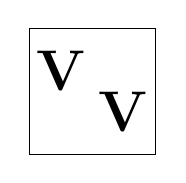
\begin{tikzpicture}
\node at (0,0) {\Huge$^\textbf{V} \,_\textbf{V}$};
\draw (-0.8,0.8) rectangle (0.8,-0.8);
\end{tikzpicture}\\[2em]

{\Large PARIS}\\[0.5em]
{\small Années 2025-2026} 

\vspace{5mm}

{\scriptsize Droits de traduction et de reproduction réservés}
\end{center}





\newpage
\onehalfspacing


% Declare paragraph level for ToC
\newlength{\cftparagraphindent}
\setlength{\cftparagraphindent}{110pt} % No indent
\newlength{\cftparagraphnumwidth}
\setlength{\cftparagraphnumwidth}{4.6em} % Adjust number width if needed

\cftsetindents{paragraph}{\cftparagraphindent}{\cftparagraphnumwidth}


\tableofcontents

\newpage


%---------------------------------
% Chapitre 1


\chapter*{Forewords}




\begin{center}
    \textit{The DCF is like a Hubble telescope — if you turn one knob a little,\\ you end up in a different galaxy} 

    ---------\\
    \textbf{Aswath Damodaran}
\end{center}

\vfill

\lettrine{A}{} valuation method always aims to determine the value of an asset or a company. However all valuation are biased : the exact pricing will never be found. The only question is how far are you from the truth and how are you biased from who you got paid. Hence, all valuation are only meant to compute an estimated value. Such a model don't need a vast amount of inputs to be useful : to keep things understandable is the key point of a valuation model. The DCF (discounted cash flows) model aims to estimate the value of an asset or business based on the present value of the expected future cash flows of that asset or business. Therefore, the assets or businesses with strong cash flows in a near future will be considered with more value than assets with later cash flows. When valuing a company, the analyst aims to determine the total value of the business — not just the equity but also the claims held by other stakeholders. The DCF model is performed under the assumption of market inefficiency : the price are not perfect and don't reflect all the available information. Market is thus expected to make mistakes in its pricing and to correct those mistakes across time with new data gathering. 





\chapter{Presentation of the model}


The core of the model relies on the discounting of future cash flow. In all this document we will use $t$ as a marker of time, and $CF_t$ as the cash flow in time $t$. The principle of the model is to discount the cash flow of the business based on grow assumption and a discount rate. Therefore, the first statement is that for a business to have a positive value, it must have positive cash flows. The cash flow we use are the free cash flows (that we could note $FCFF_t$ but we will simplify this as $CF_t$). 

\section{The inputs of the model}

Depending on valuing an asset or a firm, the inputs are not exactly the same. For valuing equity, we will use the cost of equity, whereas for valuing a firm, we will use the cost of capital. Alongside, depending on whether you use nominal or real cash flows, we will use a real or nominal discount rate. Once the discount rate is settled (it may vary across time), we must compute the current earnings and cash flows, as well as future earnings and cash flows (there we must make some assumptions about risk and growth rate). Eventually, we must estimate when the growth will stabilize and upon which parameters of risk and cash flows.   

\subsection{The discount rate}

The discount rate is a key variable in the DCF model. A small change in its estimation may lead to a significant variation in the final result. The keystone for an accurate estimation of the discount rate is coherence with the type of cash flows used in the model. Here are some principles of consistency : 

\begin{enumerate}[label=(\alph*)]
    \item \textit{Cash flow consistency} : if the discounted cash flows are cash flows to equity then the appropriate discount rate is a cost of equity. If the cash flows are free cash flows to the firm then we must use the cost of capital.

    \item \textit{Currency consistency} : The discount rate must be estimated in the same currency than cash flows.

    \item  \textit{Nominal and real consistency} : The discount rate have to be real or nominal depending on which are the cash flows.
\end{enumerate}

To value a firm we will therefore use the weighed average cost of capital ($WACC$) that is computed through the cost of equity and the cost of debt. The $WACC$ is computed using the formula : 
\begin{multline}
        WACC = \text{Cost of equity}  \times \frac{\text{Equity}}{\text{Debt + Equity}} \\+ \text{Cost of debt} \times \frac{\text{Debt}}{\text{Debt + Equity}} \times (1-t)
\end{multline}
where $t$ is the marginal tax rate on corporate income\footnote{This is a non-sense in France, take $(1-t) = 1$}.


\subsubsection{The cost of equity}

The cost of equity (CoE) is the return, as a rate, that investors require for investing in a company's equity (its shares), given the risk they are taking compared to a risk-free investment. Therefore, the cost of equity increase with investment risk profile. There are different models to compute the cost of equity $E_r$, most popular one being the Capital Asset Pricing Model (CAPM). In this model, the cost of equity is comuted by the formula : 
\begin{equation}
    E_r = r_f +\beta(r_m - r_f)
\end{equation}
where $r_f$ is the risk free rate\footnote{The risk-free rate is the theoretical return on an investment that carries zero risk of financial loss.
In practice, it represents the interest rate an investor would expect from a completely safe investment over a given period.}, the greek $\beta$ is the sensitivity of the asset returns to the returns of the overall market portfolio. Thus $\beta$ quantifies the systematic (non-diversifiable) risk of the asset relative to the market. Finally, $r_m$ is the  expected return of the market portfolio, representing the weighted average return of all investable assets in the economy ; together with $r_f$ they represent the market risk premium : $(r_m - r_f)$. In practice we use short term government bond yield as the risk free rate $r_f$. The market risk premium is determined using historical risk premiums and $\beta$ is estimated by regressing stock returns against market returns. 

\paragraph{Risk free rate estimation}

Once again, the risk free rate must be in the same currency and in the same term (nominal, real) as cash flows. On a risk free asset, the actual return equals the expected return. Hence there is no variance around the expected return. For instance we use 10 year US treasury bond yield as a risk free rate for USD investment. As for EUR investment, we tend to use German 10 year treasury bond yield. A consistent approach consists in matching the scope of the yield (3,10,20 years) with the scope of the analysis. For riskier countries, or to try a more precise approach, we can use the government bond rate and 5 year CDS spread to compute an accurate risk free rate :
\begin{equation}
    r_f = \text{Bond yield} - \text{CDS default spread}
\end{equation}
we must ensure CDS spread and bond are on the same maturity ! In case the CDS default spread is not easily found, we can asses the default spread based on the local currency rating. Moreover, in the case of a strength inflation context, we can use the yield from an inflation-indexed government bond, if one exists.  

\paragraph{Market risk premium}

The market risque premium computed by $(r_m-r_f)$ is the following parameter we will study. To compute the market risk premium we will need the annual  return of a broad index (including its dividend) and of the treasury bond on that same period. We will then make the difference between both. For this reason we have to make sure we use a "gross revenue" annual return of the index. If the "Gross Revenue" return value is not computed we have to use the geometrical mean\footnote{Damoradan bolds the geometrical mean is more accurate that a linear mean for an extended period of time with volatile values} of the annual returns : 
\begin{equation}
    r_m = \bigg( \prod^n_{i=1}(1+r_i)\bigg)^\frac{1}{n}-1
\end{equation}
were all the $r_i$ are the annual return of the year $i$. Those returns must include any dividend or coupon payments. Therefore we tend to work with GR version of an index such as CAC 40 GR\footnote{\href{See more here on Euronext website}{https://live.euronext.com/fr/product/indices/QS0011131834-XPAR/market-information}}. Thus we have
\begin{equation}
    r_i = \frac{\text{Final value GR}_i}{\text{Initial value GR}_i} -1
\end{equation}
Otherwise, if we don't work with a Gross Revenu version of the index we must add the received payments : 
\begin{equation}
    r_i = \frac{\text{Final value} +  \text{Dividends}}{\text{Initial value}} -1
\end{equation}



Considering the market index we must alway look for the longest range of data (as far as we can go in the past). However, as for the governmental bond we should use the same risk free rate $r_f$, therefore often a 5 or 10 years range. Eventually we can compute the market risk premium : 
$$
\text{Market Risk Premium} = r_m - r_f
$$

\paragraph{The greek beta}

The parameter $\beta$ measures how sensitive a company’s returns are to movements in the overall market. The standard procedure to estimate $\beta$ is to regress stock return $r_j$ against the market return $r_m$, which gives : 
\begin{equation}
    \forall\,j\in \mathbb{N},\,\, r_j = a+b\times r_m
\end{equation}
where $a$ is the intercept and $b$ is the slope of the regression model. The greek $\beta$ is simply the slope of the regression : $\beta = b$.  However we must be careful about the downsides of such a model. Indeed, the $\beta$ is not stable across time, it has a high standard error, and varies upon the selected index used for the regression. We can conclude from the regression that :
\begin{table}[H]
    \centering
    \begin{tabularx}{\textwidth}{cX}
        \toprule
        $\beta$ & \textbf{Stock behavior relative to the market} \\
        \midrule
        $\beta = 1$ & The stock moves the same as the market \\ 
        $\beta > 1$ & The stock is more volatile than the market \\
        $\beta < 1$ & The stock is less volatile than the market \\
        $\beta < 0$ & The company moves oppositely to the market \\
        \bottomrule
    \end{tabularx}
    \caption{Stock behavior relative to the market according to $\beta$ value}
    \label{tab:my_label}
\end{table}


The $\beta$ of a company is determined by three mains levers or factors that are \textit{1)} product or service type, \textit{2)} operating leverage and \textit{3)} the financial leverage. All leverage have their own implications : 

\vspace{10cm}

\begin{itemize}
    \item \textit{Nature of product or services}
    \begin{itemize}
    \item Cyclical companies should have higher betas than non-cyclical companies

    \item Luxury brands should have a higher beta than basic brands

    \item High priced goods and services should have a higher beta that low prices goods

    \item Growth firm should have a higher beta
    \end{itemize}

    \item \textit{Operating leverage}
    \begin{itemize}
        \item Firms with high structural/fixed costs should have a higher beta (because higher fixed costs increase exposure to risk)

        \item Smaller firms should have a higher beta than larger firms
    \end{itemize}

    \item \textit{Financial leverage}

    \begin{itemize}
        \item Firms with high debt should have a higher beta (because debt creates a fixed cost, interest expenses, that increases exposure to market risk)
    \end{itemize}
    
\end{itemize}

Consequently, given  the $\beta$ include leverage by debt, we call the $\beta$ obtained by regression the "levered beta" or the "equity beta". However, Damodaran reckons this beta may not be accurate enough due to noise and time instability, especially for small companies or firms that changed their core business. Instead, Damodaran advises to compute an unlevered version of $\beta$ that he notes $\beta_u$. This beta neutralize the debt lever effect and allows to compare firms with different debt, on their core business risk profile. We compute the unlevered beta using the formula : 
\begin{equation}
   \displaystyle \beta_u = \frac{\beta}{1+\frac{(1-t)D}{E}} 
\end{equation}
where $t$ is the marginal corporate tax rate\footnote{This is aplicable only if the tax rate depend upon the profit of the company. Otherwise $t$ is just the corporate tax rate}. 

As for small companies, Damodaran advises a reversed approach : the bottom-up Betas.  In that sens, we first identify the branch of businesses the firm operates in. The second step is to find publicly traded firms in each of these business and obtain their regression betas. We compute the simple average across theses regression betas to get an average beta. Finally, we unlever this average beta using the average debt-to-equity ratio across the public firm in the selected sample thanks to the formula (1.8). The following step, is to determine to what extend the different businesses the firm is involved in are participating in revenue (or EBITDA). The goal here is to get a ratio or a percentage for each line of business. Then the step four is to compute a weighted average of the unlevered betas of the different businesses (from step 2) using the weight from step 3. This results in a bottom-up unlevered beta. Eventually, we compute the levered beta for the firm using the formula : 
\begin{equation}
    \beta_L =  \beta_u \times \bigg( 1 - \frac{(1-t)D}{E}\bigg)
\end{equation}
 The advantage of such an approach is the possibility to adjust year-to-year the debt to equity ratio and the weighting of the business lines. 
 
 However, using beta  to compute the cost of equity for a private firm will always underestimate the cost of equity for that private firm. This is due to the fact that beta measures market (systematic) risk\footnote{Systematic risk is the portion of an asset’s total risk that is caused by factors affecting the entire market or economy and cannot be eliminated through diversification. It is also called market risk or non-diversifiable risk and driven by macroeconomic variables such as interest rates, inflation, economic growth, political instability, natural disasters. It affects all companies, although not equally (some sectors are more sensitive).}, i.e. the risk that matters to a diversified investor. But private firm owners are usually not diversified : a private business owner is exposed to total risk — both market risk and company-specific risk.  So, using a beta-based cost of equity (which only prices systematic risk) assumes the investor is diversified — which is not will underestimate risk profile by capturing only systematic risk that is, by definition, smaller than total risk. To adjust the beta to reflect total risk rather than market risk it is rather simple since the determination coefficient ($R^2$) of the regression measures the proportion of the risk that is market risk :
 \begin{equation}
      \beta_{total} = \frac{\beta}{\sqrt{R^2}} = \frac{\beta}{\sqrt{\rho^2}}
 \end{equation}
where $\rho$ is the correlation coefficient between stock returns of the company (or sector) and the returns of the overall market. Therefore $\rho$ asses how much the asset moves with the market, but unlike beta, it doesn't scale by volatility — it’s a pure measure of co-movement. For $R_i$ the serie of returns for the firm and $R_m$ a serie of market return we have then 
\begin{equation}
    \rho = \frac{\operatorname{cov}(R_i,R_m)}{\sigma_i\times\sigma_m} \qquad \quad \rho = \frac{\beta}{\displaystyle\frac{\sigma_i}{\sigma_m}}
\end{equation}
where $\sigma$ are the standard deviation for the market or the firm. The $\beta_{total}$ can be then used in the CAPM model !

\paragraph{Adressing risk profile}

In another hand, we can modify slightly the CAPM model to get a more accurate view of  the risk profile of the company. This works with the country Equity Risk Premium (ERP) that is estimated by 5 year CDS spread on the given country. The second parameter we will need is the US premium. There is two way to compute this premium : the first one (historical premium) is to to make a geometrical mean on the period of the 10 year T-bond yield and of the stock yield over the most extended period possible, and to substract the T-bond yield mean to the stock one ; the second way (implied premium) will require the level of country index (ex. CAC40, S\&P500, DAX...) $L_{index}$, the T-bond rate $B_{rate}$, the expected growth rate $g$ in the index cash flows for the next 5 years\footnote{The cash flows are the dividends plus stock buybacks of the entire index (share repurchases by the company)} that will allows us to get a 5-year-long serie of cash flows based on the first year cash flows ; and the perpetual growth rate $g_{perpetual}$. Then  by discounting the level of the index is given by :
\begin{equation}
L_{index} = \sum^5_{t=1}\frac{CF_t}{(1+r)^t} + \displaystyle\frac{\frac{CF_6}{r-g_{perpetual}}}{(1+r)^5}
\end{equation}
the we must solve for $r$ (the only way is by trial and error). Once $r$ is found, we can compute the implied risk premium : 
\begin{equation}
    \text{Implied Risk Premium} = r - r_f
\end{equation}
based on this implied risk premium, (particularly useful for the US), we can compute some variation of the CPAM model to adress different risk profiles : 

\begin{enumerate}
    \item \textit{Variation 1} : Assume that every company in the country is equally exposed to country risk. In this case :
    \begin{equation}
        E_r = r_f + \text{Country spread} +\beta \times \text{US premium}
    \end{equation}


    \item \textit{Variation 2} : Assume that a company’s exposure to country risk is similar to its exposure to other market risk.
    \begin{equation}
        E_r = r_f + \beta\times(\text{US premium}+\text{Country spread})
    \end{equation}

    \item \textit{Variation 3} : Treat country risk as a separate risk factor and allow firms to have different exposures to country risk (perhaps based upon the proportion of their revenues come from non-domestic sales) 
    \begin{equation}
        E_r = r_f + \beta \times \text{US premium} + \sum_{i=1}^n(\lambda_i \times \text{Country spread}_i)
    \end{equation}
    where $\sum_{i=1}^n\lambda_i = 1$ based on the proportion of each country in the firm's activity.
\end{enumerate} 

Finally, Damodaran advises rather to use implied ERP in the CPAM model than the historical market risk premium because implied ERP reflects what the market demands today for equity risk, based on actual prices and expected future cash flows ; and it avoids arbitrary choices like "how far back" and "T-bills or T-bonds?". Therefore, we can compute the cost of equity based on the CPAM model : 
\begin{equation}
    E_r = r_f + \beta\times \text{Implied ERP}
\end{equation}

\paragraph{Conclusion}

The cost of equity is computed by the risk free rate $r_f$ (that has to be in the same currency and in the same term real or nominal as the cash flows) ; the $\beta$ (we will preferably use the bottom-up beta based upon other firms in the business) ; and the risk premium (either the historical risk premium or the implied risk premium that is better according to Damodaran). Once the cost of equity is found, we can start the next step : to compute the cost of debt. 

\subsubsection{The cost of debt}

The cost of debt is the rate at which we can borrow at currently, It will reflect not only our default risk but also the level of interest rates in the market. There are two main approaches to estimate the cost of debt. The first one is looking up the yield to maturity on a straight bond outstanding from the firm. The limitation of this approach is that very few firms have long term straight bonds that are liquid and widely traded. The second one is looking up the rating for the firm and estimating a default spread based upon the rating. While this approach is more robust, different bonds from the same firm can have different ratings. we have to use a median rating for the firm. When in trouble (either because we  have no ratings or multiple ratings for a firm), we must estimate a synthetic rating for the firm and the cost of
debt based upon that rating.



\end{document}

% CAPM variation



% Beta regression

\begin{figure}[h!]
\centering
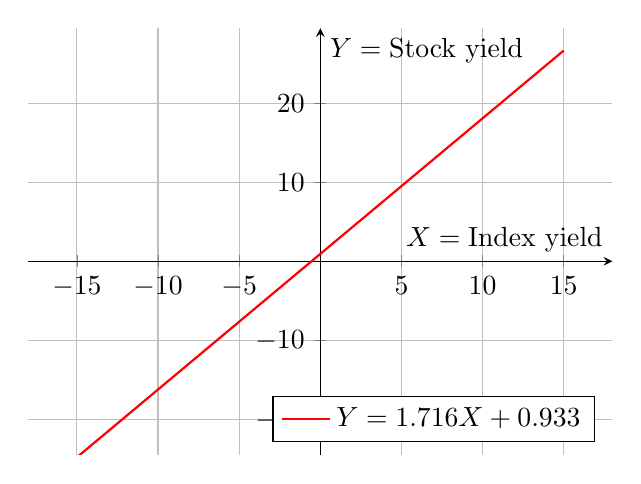
\begin{tikzpicture}
\begin{axis}[
    xlabel={$X = \text{Index yield}$},
    ylabel={$Y = \text{Stock yield}$},
    grid=both,
    axis lines=middle,
    xmin=-15, xmax=15,
    ymin=-20, ymax=25,
    width=9cm, height=7cm, % Taille réduite ici
    enlargelimits=true,
    samples=100,
    domain=-15:15,
    legend pos=south east
]

% Droite de régression
\addplot[thick, red] {1.716*x + 0.933};
\addlegendentry{$Y = 1.716X + 0.933$}

\end{axis}
\end{tikzpicture}
\caption{Regression between stock and index return}
\end{figure}
